\begin{pastexam}[label={px:df3-114-ds-03}]{地方三等資訊處理 114 年 第三題}
（申論；30 分）

二元搜尋樹（binary search tree）是一種常見的資料結構。
\begin{enumerate}[leftmargin=2.2em]
\item[㈠] 請將 50, 30, 70, 20, 40, 60, 80 依序插入一個二元搜尋樹，然後再從該二元樹刪除 50，並畫出每個數字
放入或刪除後的二元搜尋樹。（10 分）
\item[㈡] 以下陣列儲存了一個二元搜尋樹，根節點為 A(1)，若針對該二元樹刪除 40，請顯示該陣列的變化。（5 分）
\begin{center}
\small
\begin{tabular}{|c|*{17}{c|}}
\hline
i & 1 & 2 & 3 & 4 & 5 & 6 & 7 & 8 & 9 & 10 & 11 & 12 & 13 & 14 & 15 & 16 & 17 \\
\hline
A(i) & 40 & 30 & 70 & 10 & -- & 50 & 90 & -- & 20 & -- & -- & -- & 60 & 80 & -- & -- & -- \\
\hline
\end{tabular}
\end{center}
\item[㈢] 以下陣列儲存了一個二元搜尋樹，根節點為 A(1)，若針對該二元樹刪除 30，請顯示該陣列的變化。（5 分）
\begin{center}
\small
\begin{tabular}{|c|*{17}{c|}}
\hline
i & 1 & 2 & 3 & 4 & 5 & 6 & 7 & 8 & 9 & 10 & 11 & 12 & 13 & 14 & 15 & 16 & 17 \\
\hline
A(i) & 40 & 30 & 70 & 10 & -- & 50 & 90 & -- & 20 & -- & -- & -- & 60 & 80 & -- & -- & -- \\
\hline
\end{tabular}
\end{center}
\item[㈣] 以下陣列儲存了一個二元搜尋樹，根節點為 A(1)，請列舉可依序插入的五個數值，使得該二元樹成為完整
二元樹（full binary tree）。（10 分）
\begin{center}
\small
\begin{tabular}{|c|*{17}{c|}}
\hline
i & 1 & 2 & 3 & 4 & 5 & 6 & 7 & 8 & 9 & 10 & 11 & 12 & 13 & 14 & 15 & 16 & 17 \\
\hline
A(i) & 40 & 30 & 70 & 10 & -- & 50 & 90 & -- & 20 & -- & -- & -- & 60 & 80 & -- & -- & -- \\
\hline
\end{tabular}
\end{center}
\end{enumerate}
\end{pastexam}

\begin{pastsoln}
刪除有兩個子節點的節點時，本題都用中序\textbf{後繼}（右子樹的最小值）取代，和資結書第~9.2~節一致；
用前驅（左子樹的最大值）也對，結果不同，下面也附上。

\textbf{㈠ 依序插入再刪除 50。} 每次從根開始比較，小往左、大往右，走到空位放下（資結書第~9.2~節）：
\begin{center}
\begin{tikzpicture}[
    every node/.style={circle, draw, minimum size=6.5mm, inner sep=0pt, font=\scriptsize},
    lab/.style={draw=none, rectangle, font=\scriptsize},
    level distance=9mm,
    level 1/.style={sibling distance=16mm},
    level 2/.style={sibling distance=8.5mm}]
\node at (0,0) {50};
\node[lab] at (0,-2.6) {插入 50};
\begin{scope}[xshift=2.3cm]
\node {50} child {node {30}} child[missing];
\node[lab] at (0,-2.6) {插入 30};
\end{scope}
\begin{scope}[xshift=5.1cm]
\node {50} child {node {30}} child {node {70}};
\node[lab] at (0,-2.6) {插入 70};
\end{scope}
\begin{scope}[xshift=8.3cm]
\node {50} child {node {30} child {node {20}} child[missing]} child {node {70}};
\node[lab] at (0,-2.6) {插入 20};
\end{scope}
\begin{scope}[xshift=11.6cm]
\node {50} child {node {30} child {node {20}} child {node {40}}} child {node {70}};
\node[lab] at (0,-2.6) {插入 40};
\end{scope}
\begin{scope}[xshift=1.6cm, yshift=-3.6cm]
\node {50} child {node {30} child {node {20}} child {node {40}}} child {node {70} child {node {60}} child[missing]};
\node[lab] at (0,-2.6) {插入 60};
\end{scope}
\begin{scope}[xshift=6cm, yshift=-3.6cm]
\node {50} child {node {30} child {node {20}} child {node {40}}} child {node {70} child {node {60}} child {node {80}}};
\node[lab] at (0,-2.6) {插入 80};
\end{scope}
\begin{scope}[xshift=10.4cm, yshift=-3.6cm]
\node {60} child {node {30} child {node {20}} child {node {40}}} child {node {70} child[missing] child {node {80}}};
\node[lab] at (0,-2.6) {刪除 50（用後繼 60）};
\end{scope}
\end{tikzpicture}
\end{center}
刪除 50：50 有兩個子節點。 後繼是右子樹 \{70, 60, 80\} 的最小值 60，60 是葉節點，直接拿下來放到根的
位置，70 的左子變空。 若用前驅 40（左子樹最大值，也是葉節點），結果是根 40，左子 30 只剩左子 20，
右子樹 70(60, 80) 不變。

\textbf{陣列裡的樹（㈡ ㈢ ㈣ 共用）。} A($i$) 的左子在 A($2i$)、右子在 A($2i+1$)（資結書第~7.2.1~節）：
根 40；A(2)$=$30 的左子 A(4)$=$10，右子 A(5) 空；10 的右子 A(9)$=$20；A(3)$=$70 的左子 A(6)$=$50、右子
A(7)$=$90；50 的右子 A(13)$=$60；90 的左子 A(14)$=$80。
\begin{center}
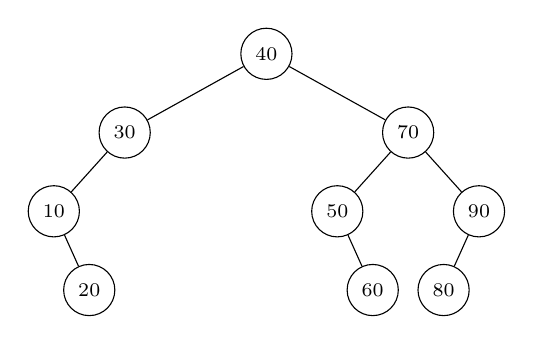
\begin{tikzpicture}[
    every node/.style={circle, draw, minimum size=6.5mm, inner sep=0pt, font=\scriptsize},
    level distance=10mm,
    level 1/.style={sibling distance=36mm},
    level 2/.style={sibling distance=18mm},
    level 3/.style={sibling distance=9mm}]
\node {40}
  child {node {30} child {node {10} child[missing] child {node {20}}} child[missing]}
  child {node {70} child {node {50} child[missing] child {node {60}}} child {node {90} child {node {80}} child[missing]}};
\end{tikzpicture}
\end{center}
陣列存法的麻煩是：一個節點往上移，它整棵子樹的每個節點編號都要跟著改（編號 $j$ 的節點往上一層，
新編號要依它是左子或右子重新計算）。

\textbf{㈡ 刪除 40。} 40 是根，有兩個子節點。 後繼是右子樹的最小值：從 70 往左到 50，50 沒有左子，
所以後繼是 50（在 A(6)）。 把 50 放到 A(1)；50 原本的右子樹（只有 60）接到 50 原本的位置，60 從
A(13) 移到 A(6)。
\begin{center}
\small
\begin{tabular}{|c|*{17}{c|}}
\hline
i & 1 & 2 & 3 & 4 & 5 & 6 & 7 & 8 & 9 & 10 & 11 & 12 & 13 & 14 & 15 & 16 & 17 \\
\hline
A(i) & \textbf{50} & 30 & 70 & 10 & -- & \textbf{60} & 90 & -- & 20 & -- & -- & -- & \textbf{--} & 80 & -- & -- & -- \\
\hline
\end{tabular}
\end{center}
變動的是 A(1)：40 → 50、A(6)：50 → 60、A(13)：60 → 空。 （用前驅 30 的話：A(1) 放 30，30 的左子樹
10(--, 20) 上移一層，A(2)$=$10、A(5)$=$20、A(4)、A(9) 變空。）

\textbf{㈢ 刪除 30。} 30 只有左子樹（以 10 為根，10 的右子是 20），屬於「只有一個子節點」的情況：
整棵左子樹往上接到 30 的位置。 10 從 A(4) 移到 A(2)；20 是 10 的右子，從 A(9) 移到 A(2$\cdot$2$+$1)$=$A(5)。
\begin{center}
\small
\begin{tabular}{|c|*{17}{c|}}
\hline
i & 1 & 2 & 3 & 4 & 5 & 6 & 7 & 8 & 9 & 10 & 11 & 12 & 13 & 14 & 15 & 16 & 17 \\
\hline
A(i) & 40 & \textbf{10} & 70 & \textbf{--} & \textbf{20} & 50 & 90 & -- & \textbf{--} & -- & -- & -- & 60 & 80 & -- & -- & -- \\
\hline
\end{tabular}
\end{center}

\textbf{㈣ 插入五個數變成完整二元樹。} 先處理題目的用詞：原卷寫「完整二元樹（full binary tree）」。
若照字面的 full binary tree，有兩種意思，都做不到：每個節點的子節點數都是 0 或 2 的樹，節點數一定是
奇數，而 $9 + 5 = 14$ 是偶數；每一層都滿的樹，4 層要 15 個節點，不是 14 個。 所以這裡採中文「完整二元樹」
的意思，也就是 complete binary tree（資結書第~7.1~節）：除了最後一層都是滿的，最後一層的節點靠左排。
14 個節點的完整二元樹，陣列 A(1)--A(14) 恰好全部有值。

目前 A(1)--A(14) 空著的是 A(5)、A(8)、A(10)、A(11)、A(12)，正好 5 格，新插入的五個數要剛好落在這五格。
各格的鍵值範圍由它在樹上的位置決定：
\begin{itemize}
\item A(5)：30 的右子，在 30 和 40 之間。
\item A(8)：10 的左子，小於 10。
\item A(10)、A(11)：A(5) 的左、右子，分別在 30 和 A(5) 之間、A(5) 和 40 之間，所以 A(5) 要先插入。
\item A(12)：50 的左子，在 40 和 50 之間。
\end{itemize}
一組答案：依序插入 \textbf{35, 5, 32, 38, 45}。
\begin{itemize}
\item 35：$< 40$ 往左到 30，$> 30$ 往右，A(5) 空，放在 A(5)。
\item 5：$< 40$、$< 30$、$< 10$，放在 10 的左子 A(8)。
\item 32：$< 40$、$> 30$ 到 35，$< 35$，放在 A(10)。
\item 38：$< 40$、$> 30$ 到 35，$> 35$，放在 A(11)。
\item 45：$> 40$ 到 70，$< 70$ 到 50，$< 50$，放在 A(12)。
\end{itemize}
結果 A(1)--A(14) 依序是 40, 30, 70, 10, 35, 50, 90, 5, 20, 32, 38, 45, 60, 80，是一棵 14 個節點的完整二元樹，
也仍然是二元搜尋樹（中序 5, 10, 20, 30, 32, 35, 38, 40, 45, 50, 60, 70, 80, 90 遞增）。 只要滿足上面的範圍和
「A(5) 比 A(10)、A(11) 先插入」，其他數值和順序也可以。
\end{pastsoln}
